%%%%%%%%%%%%%%%%%%%%%%%%%%%%%%%%%%%%%%%%%
% Simple Sectioned Essay Template
% LaTeX Template
%
% This template has been downloaded from:
% http://www.latextemplates.com
%
% Note:
% The \lipsum[#] commands throughout this template generate dummy text
% to fill the template out. These commands should all be removed when 
% writing essay content.
%
%%%%%%%%%%%%%%%%%%%%%%%%%%%%%%%%%%%%%%%%%

%----------------------------------------------------------------------------------------
%	PACKAGES AND OTHER DOCUMENT CONFIGURATIONS
%----------------------------------------------------------------------------------------

\documentclass[12pt]{article} % Default font size is 12pt, it can be changed here

\usepackage{geometry} % Required to change the page size to A4
\geometry{a4paper} % Set the page size to be A4 as opposed to the default US Letter

\usepackage{graphicx} % Required for including pictures

\usepackage{float} % Allows putting an [H] in \begin{figure} to specify the exact location of the figure
\usepackage{wrapfig} % Allows in-line images such as the example fish picture

\usepackage{lipsum} % Used for inserting dummy 'Lorem ipsum' text into the template

\linespread{1.2} % Line spacing

%\setlength\parindent{0pt} % Uncomment to remove all indentation from paragraphs

\graphicspath{{./Pictures/}} % Specifies the directory where pictures are stored

%%%%%%%%% PUT BY ME %%%%%%%%%%%%%%%%%%
\usepackage[usenames,dvipsnames]{xcolor}

\usepackage{caption}
\usepackage{subcaption}

\usepackage{tikz}
\usetikzlibrary{decorations.markings}

\usepackage[ruled,vlined]{algorithm2e}

\usepackage{amsmath}

\usepackage{pgfplots}

\newcommand{\Olivier}[1]{\footnote{\color{green}Olivier: #1}}
\newcommand{\Berenger}[1]{\footnote{\color{blue}Berenger: #1}}
\newcommand{\TODO}[1]{\textbf{\color{red}Todo: #1}}
%%%%%%%%% END PUT BY ME %%%%%%%%%%%%%%%%%%

\begin{document}

%----------------------------------------------------------------------------------------
%	TITLE PAGE
%----------------------------------------------------------------------------------------

\begin{titlepage}

\newcommand{\HRule}{\rule{\linewidth}{0.5mm}} % Defines a new command for the horizontal lines, change thickness here

\center % Center everything on the page

\textsc{\LARGE INRIA}\\[1.5cm] % Name of your university/college
\textsc{\Large HiePACS Team}\\[0.5cm] % Major heading such as course name
\textsc{\large Bordeaux}\\[0.5cm] % Minor heading such as course title

\HRule \\[0.4cm]
{ \huge \bfseries ScalFMM Periodic Model}\\[0.4cm] % Title of your document
\HRule \\[1.5cm]

\begin{minipage}{0.4\textwidth}
\begin{flushleft} \large
\emph{Author:}\\
Berenger \textsc{Bramas} \\% Your name
Olivier \textsc{Coulaud} % Your name

\end{flushleft}
\end{minipage}
~
\begin{minipage}{0.4\textwidth}
\begin{flushright} \large
%\emph{Supervisor:} \\
%\textsc{} % Supervisor's Name
\end{flushright}
\end{minipage}\\[4cm]

{\large \today}\\[1cm] % Date, change the \today to a set date if you want to be precise

{\Large \textbf{Working note}}
\vfill % Fill the rest of the page with whitespace

\end{titlepage}

%----------------------------------------------------------------------------------------
%	TABLE OF CONTENTS
%----------------------------------------------------------------------------------------

\tableofcontents % Include a table of contents

\newpage % Begins the essay on a new page instead of on the same page as the table of contents 

%%%%%%%%%%%%%%%%%%%%%%%%%%%%%%%%%%%%%%%
\section{Abstract}

The current report describes a new algorithm in order to perform an periodic Multipole Method (FMM).
This algorithm uses the usual FMM operators ($M2M$, $M2L$, $L2L$, $P2P$) why makes it kernels independent in a way explained in the later sections.
The computational cost of the method is small and is using the same error bound as the FMM.

Keywords: FMM, octree, periodic.

%%%%%%%%%%%%%%%%%%%%%%%%%%%%%%%%%%%%%%%
\section{Introduction}
The FMM is widely use to execute physical simulations with pairs interactions.
Direct approaches compute all interactions and have a complexity of $O(n^2)$.
The FMM reduce this complexity to a $O(n)$.
But many physical problems need to compute the periodic conditions.
Several solutions relies on analytical methods.

\paragraph{Type of interactions.}

In the current report we speak of potential at particle $x_i$ given by:
$$
V(x_i) = \sum_{j=0,i\neq j}^{N}{\frac{q_j}{\|x_i-x_j\|}}
$$ 
and the force on atom $x_i$ writes
$$
f(x_i) =  \sum_{j=0,i\neq j}^{N}{q_j\frac{x_i-x_j}{\|x_i-x_j\|^3}}.
$$
Finally, the total energy of the system is
$$
U = \frac{1}{2}\sum_{i=0}^{N}{q_i V(x_i)}.
$$ 

Such formulas are supported by ScalFMM.

%%%%%%%%%%%%%%%%%%%%%%%%%%%%%%%%%%%%%%%
\section{State of the art}

In APPLICATION OF FAST MULTIPOLE METHOD TO MICROMAGNETIC SIMULATION OF PERIODIC SYSTEMS, an approach is proposed but
is not using the power of FMM and the usual shape of its operators.

%%%%%%%%%%%%%%%%%%%%%%%%%%%%%%%%%%%%%%%
\section{Usual Operators}
In this section we remind the common FMM operators in an algorithm view.

\subsection{Octree}
The FMM operators rely on the spacial decomposition of the problem which is done using an octree.
The system is included in a cube where the root of the tree at level $0$ contains all the data.
Then we divide this root-cell by $2$ in each dimension which creates $2^{DIM}$ sub-cells.
We repeat the previous step until a level $L$. We have a maximum of $2^{DIM*l}$ cells at level $l$.
Some implementation subdivides a cell until a condition is respected, like for example having less than $N$ particles in each leaves.
Such approaches leads to a tree where all leaves may not be at the same level, but our method can even be applied them.

\begin{figure}[h]
\centering
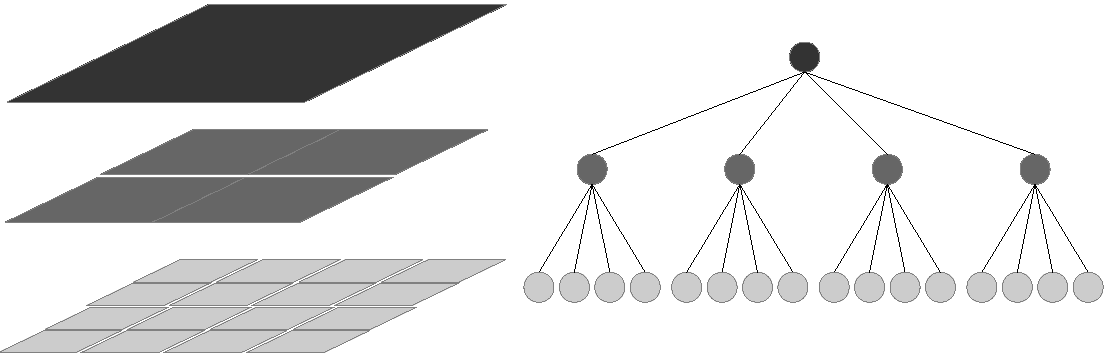
\includegraphics[scale=0.6]{Images/Octree}
\caption{$2D$ Octree}
\end{figure}

\subsection{Top Down Operators}
These operators are performing computation between a cell and its children (the cells it contains one lower level in the tree) called $M2M$ and $L2L$,
and inside leaves between cells and particles called $P2M$ and $L2P$.
Some implementation defines optimizations which make them having operators that skips level during $M2M$ or $L2L$.
But in most FMM it exists a $M2M$ (and a $L2L$) which is able to compute the interaction between a cells and its $2^{DIM}$ children.
The children are positioned at equal distance from their common parent $r$ and can be positioned using spherical coordinates:
$(r,\theta,\phi)$, with $(\theta,\phi) \in \{\pi/4,3\pi/4\} \times \{\pi/4, 3\pi/4, 5\pi/4, 7\pi/4\}$ in $3D$ and
$(r,\phi)$, with $(\phi) \in \{\pi/4, 3\pi/4, 5\pi/4, 7\pi/4\}$ in $2D$.
Depending on the level where the operator is applied, $r$ is equal to half of a cube diagonal:
$r = Diagonal/2 = \sqrt{ 3 * Edge^2 }/2 = \sqrt{ 3 * (BoxWidth/2^{l})^2 }/2$.

\begin{figure}[h]
\centering
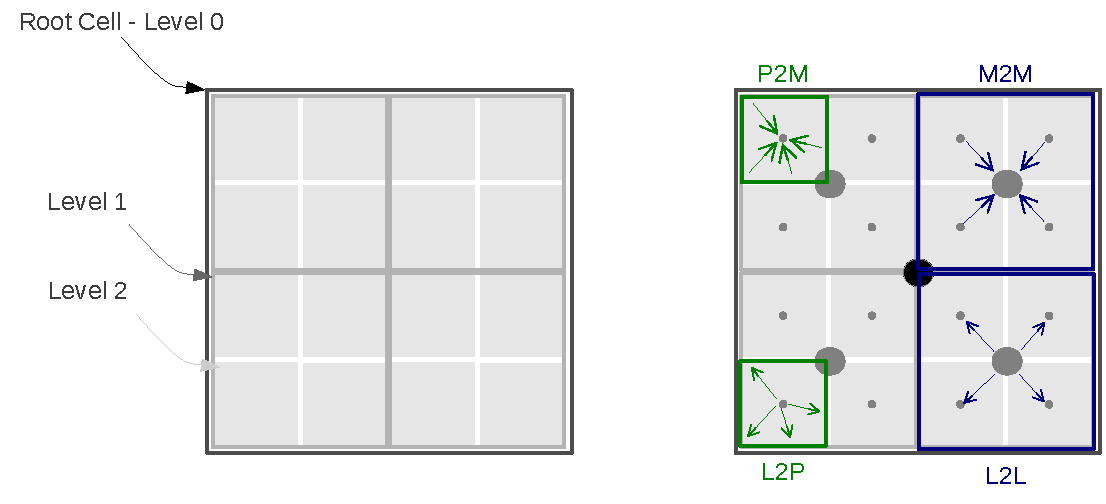
\includegraphics[scale=0.6]{Images/TopDownOperators}
\caption{Top-Down Operators}
\end{figure}

\subsection{Interactions operators}
The operators that operate on one level and do not rely on the parent or sub-cells are the $P2P$ and the $M2L$.
The $P2P$ operates between neighbors leaves. If the tree is full (each cell exists), each leaf has a number of neighbors $ng$ with
$2^{DIM} - 1 \leq ng \leq 3^{DIM}-1$.
The minimum is for leaves that are positioned in the corners.
If the octree is not full then the minimum can be $0$ since leaf may not have any neighbors.

The $M2L$ operates between a cell and what is called its interaction list.
The interaction list is composed of cells from the same level and which are not neighbors but are closed.
The closed properties is true for the cells which have their parents as neighbors respectively.
So each cell has a unique interactions list.
Depending on the position of a cell relatively to its parent, the interactions list is taken cells from $[-3;+2]$ or $[-2;+3]$ in each dimension.
In $3D$ and with a full octree, each cell has a maximum of $6^3-3^3 = 189$ interactions.
The $6^3$ is coming from the cube of size $5$ which is encapsulate all the potential interactions and the $3^3$ represents the cell itself and its neighbors.
Any FMM implementation has the capacity to compute the $M2L$ between two cell of the same level that are separated by at least one and a maximum of two in each direction.

\begin{figure}[h]
\centering
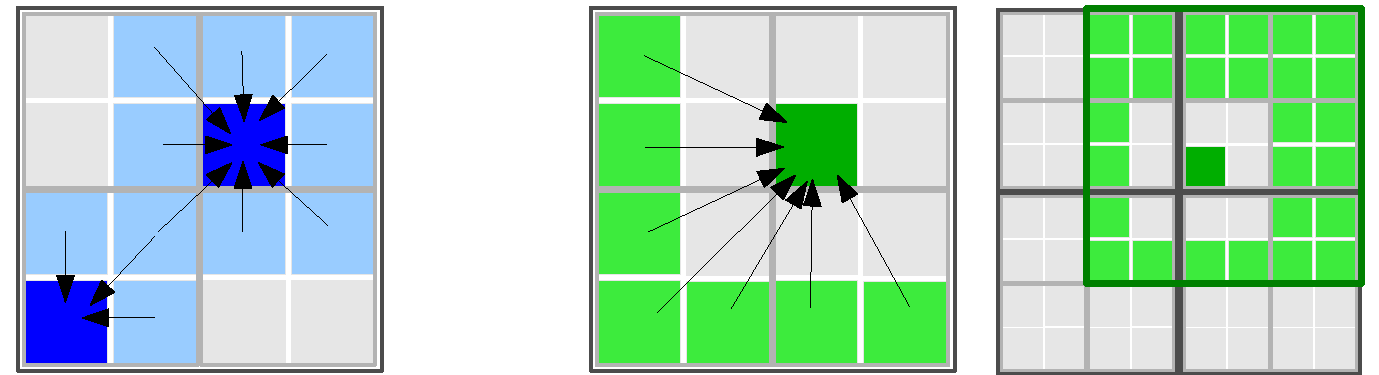
\includegraphics[scale=0.6]{Images/InteractionsOperators}
\caption{Interactions Operators, P2P (Blue), M2L (Green)}
\end{figure}

\subsection{Global view of the algorithm}
The FMM algorithm can be split in three majors parts, an upward pass, a transfer pass and a downward pass.
The upward pass is composed by the $P2M$ and the $M2M$, it centralized the information contains by each cell from leaf level to the top of the tree.
The transfer pass, composed by the $M2L$, is translating the values at each level using the interactions lists.
Then the downward pass, using $L2L$ and $L2P$, merge the results of the transfer pass and impact the leaves by starting from the root.
In the non periodic FMM, there is no computation above level $2$ since no $M2L$ happens at level $1$ because the interactions lists are empty.

In addition of these steps called the far field, we compute the near field which is the $P2P$ operators.


%%%%%%%%%%%%%%%%%%%%%%%%%%%%%%%%%%%%%%%
\section{Virtual Repetition}

When using periodicity, a cell or a leaf can have its interactions or neighbors lists extended.
In fact, when working with periodicity the simulation box should be repeated.
A cell on the border or separated by one cell from the border should have interactions from the other side of the box.
In the next paragraph we supposed when speaking about interactions or neighbors lists that they are a periodic lists.

\begin{figure}[h]
\centering
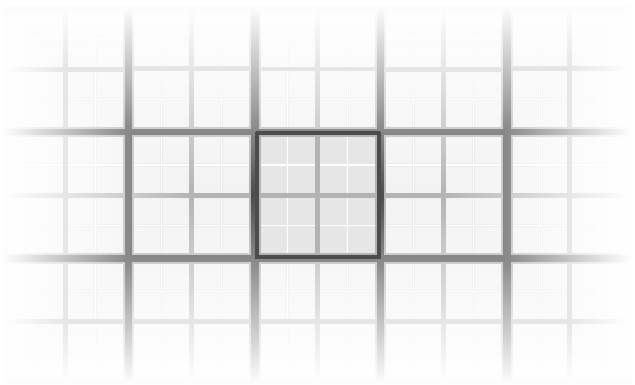
\includegraphics[scale=0.6]{Images/Repetitions}
\caption{Repetitions of the simulation box create new neighbors}
\end{figure}

\subsection{Periodicity during normal pass}
During the upward pass the periodicity does not change the operators.
In fact, they are operate between cells and sub-cells.

Whereas, the transfer pass ($M2L$ and $P2P$) should not work with periodic lists.
The normal FMM stops at level $2$ because interactions lists are empty at level $1$.
By doing this, it makes a repetition of original box $rep(2) = 1/2$.
If we use the upward pass, transfer pass and downward pass at level $1$ then $rep(1) = 1$.
In fact, at level $1$ the periodic interactions lists are not empty and the $M2L$ at level $1$ is covering the neighbors of our root.
It is important to have in mind that without any special operation the box is already repeated once it we go at level $1$ and use periodic lists.

\begin{figure}[h]
\centering
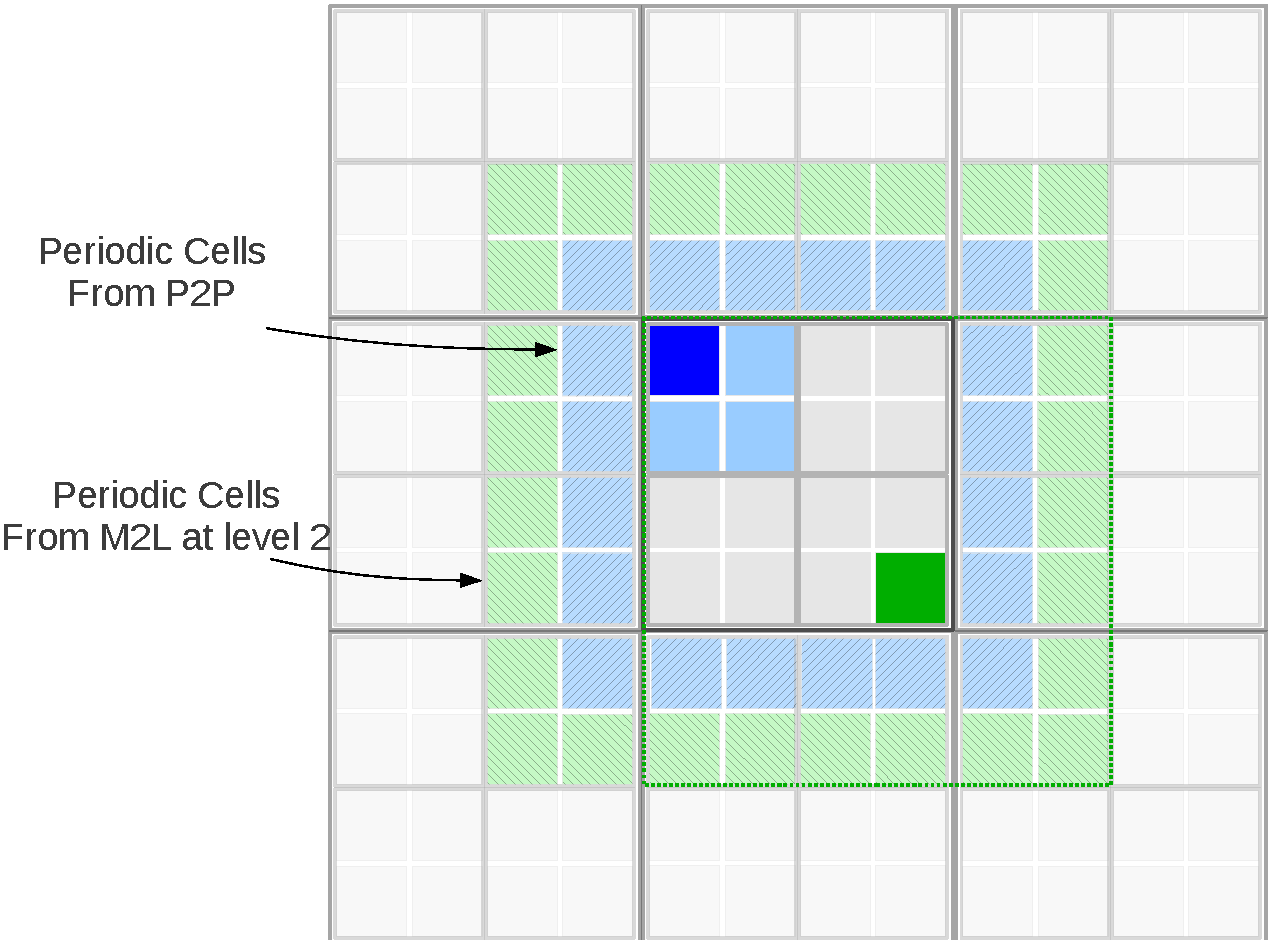
\includegraphics[scale=0.35]{Images/PeriodicL2}
\caption{Extension of the box with a periodicity until level $2$}
\end{figure}

\subsection{Periodicity at root level}
If the $M2M$ goes until the root at level $0$, the root cell is containing all the information of the entire tree.
Using this cell we can perform a $M2L$ from $-3$ to $3$ by using it same cell inside the interactions lists.
This $M2L$ will not compute the interaction with the neighbors cells, but this has been already done.
We then have a repetition of $2$ cells in each direction so it like having a grid of $(2*2)+1$ and working on the cell in the middle.
Finally we can compute the downward pass from level $0$ to the leaves.

\begin{figure}[h]
\centering
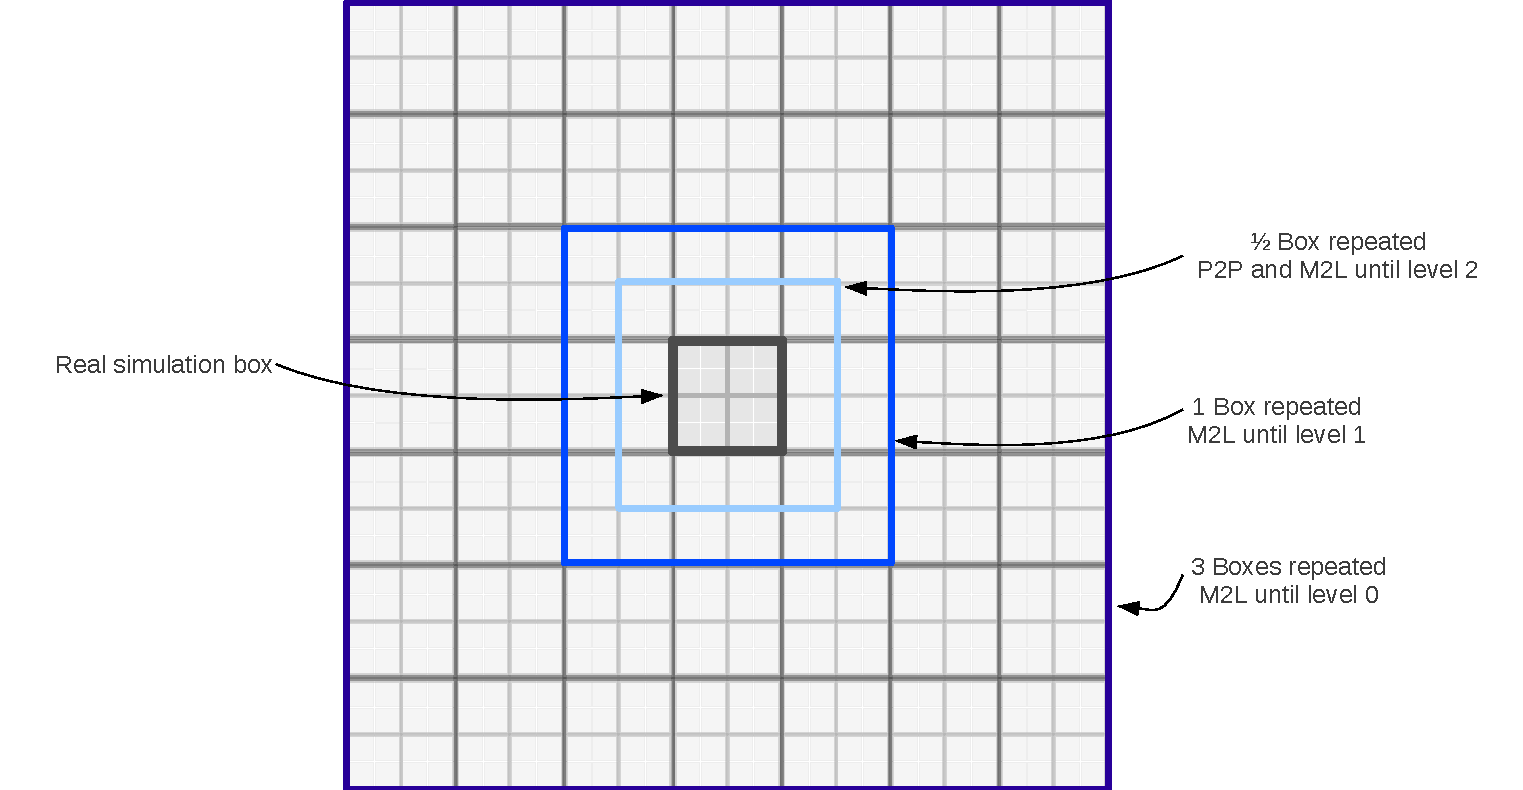
\includegraphics[scale=0.45]{Images/PeriodicL0}
\caption{Extension of the box with a periodicity until level $0$}
\end{figure}

\subsection{Periodicity above the root}
In the previous paragraph we stopped the operation at level $0$.
But the key idea of the periodic algorithm is to continue with the usual operators above the level $0$ of the tree.

If we compute the $M2L$ between $[-3;+3]$ at level $0$ it is then impossible to continue with the usual operators.
In fact, the $M2L$ is covering what sub-cells do not cover and should let too far cells to upper $M2L$.
The $M2L$ at level $0$ has to be limited to $[-3;+2]$ or $[-2;+3]$ in each direction.

This choice is made by choosing where does our current root is situated relatively to its parent.
Any choice can be made, but we consider that the root cell it at position $(1,1,1)$ relatively to its parent.
So when performing the $M2L$ at level $0$ the repetition of the box is not odd and so it is not equilibrate.
It is similar as having a grid of width $6$ and working on the cell of coordinate $(4,4,4)$.
We can continue to perform similar operations, $M2M$ followed by $M2L$ and considering that our working cell is in $(1,1,1)$ relatively to its parent.

Then, at the last level above the root, the final $M2L$ should be perform by considering that the working cell is in position $(0,0,0)$ relatively to its parent.
This put our working cell in the middle of the grid.

It remains that the repetition is not symmetric.
In fact, the grid has a width of $(6*2^d)$ which is odd.
There are $(6*2^d)/2$ repetition in one side and $((6*2^d)/2)-1$ in the other side for all the dimensions.
The have a perfect symmetric periodicity we need to add a border.

\begin{figure}[h]
\centering
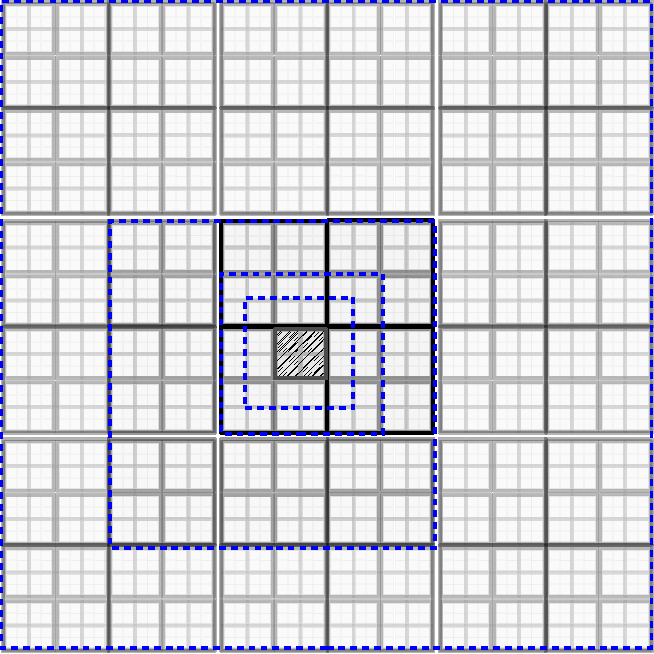
\includegraphics[scale=0.45]{Images/PeriodicL-1}
\caption{Extension of the box with a periodicity until level $-1$ without border}
\end{figure}

We can group the root cell to perform a $M2M$ from level $0$ to level $-1$.
The results contains the information of a box which is nothing more than our original box repeated $2$ times in each direction.
Again, we can do a $M2L$ at level $-1$ and we choose that our cell is at position $(0,0,0)$ relatively to its parent.
These operations can be repeated until we have enough repetition.

Every time we perform a $M2M$ $d$ levels above $0$ we create a new cell which contain $2^d$ times our original box.
Then when we perform a $M2M$ at a level we repeat the cell from $-2$ to $3$ in any direction.
So at $d$ levels above $0$ performing a $M2L$ leads to create a repetition of $6*2^d$ original box in all the directions.
So we create a grid of size $(6*2^d)^3$ and we are working on the center cell at position $((6*2^d)/2,(6*2^d)/2,(6*2^d)/2)$.


\subsection{Adding a border}

THIS IS NOT USE ANYMORE!

After having proceed $d$ levels above $0$, a border of the simulation box is missing.
To take into consideration this border, we need to use the root cell and create all the configuration in order to have create
cells one levels above $d$ which contains all the information.
Then we can apply a final $M2L$ between those cells and our working cell.

In $2D$ there are three kinds of border cells: the horizontal border, the vertical border and the angle.
In $3D$ there are seven kinds of border cells: the top, the side, the back and the four different links between them.
More generally, there are $DIM$ different sides and $2^{DIM-1}$ different connexion between sides.

Computing the cell which represent a side is done in $d-1$ $M2M$.
Each of this $M2M$ is computing the relation between one or two sub-cells and their parent.

\begin{figure}[h]
\centering
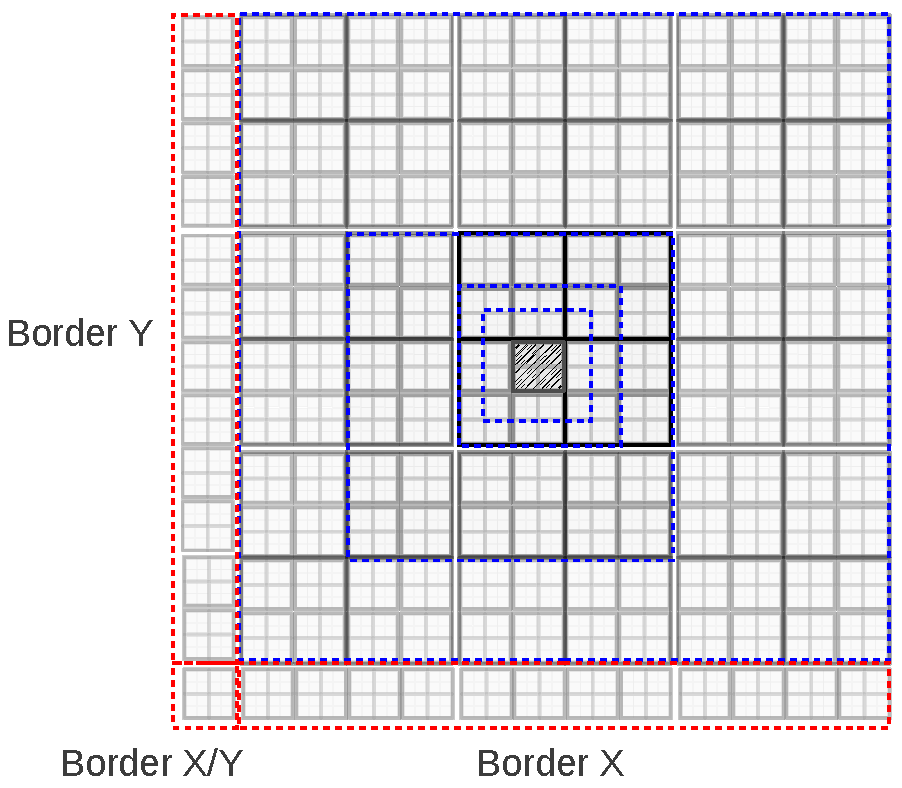
\includegraphics[scale=0.45]{Images/Border}
\caption{Extension of the box with a periodicity until level $-1$ with border}
\end{figure}

\subsection{Limiting the periodicity direction}

If the simulation needs that the periodicity is limited in some direction, for example $(+X,+-Y,No \, Z)$, the only changes is in the construction to the periodic lists including those made above the root.
Then, during the addition of the border only the periodic directions have to be applied.

%%%%%%%%%%%%%%%%%%%%%%%%%%%%%%%%%%%%%%%
\section{Theoretical repetition}

The periodic-algorithm does not allow to choose a specific grid size.
The only parameter $D$ is the number of level above the root of the box where the algorithm is applied.
As it has been illustrated the final grid size has a width of $dim = 2^{Abs(D)+2}$

\begin{center}
\begin{tabular}{ | c | c | }
 \hline                 
   D & Grid Dim \\ \hline
   1 & 3 \\
   0 & 4 \\
   1 & 8 \\
   5 & 32 \\
   20 & 1 048 576 \\
 \hline  
 \end{tabular}
\end{center}

\subsection{Cost above the root}
We determine the cost of the periodicity in term of FMM operators.
The following cost is based on a full octree.

There are $2^{DIM}$ $M2M$, $1$ $L2L$, and $6^{DIM}-3^{DIM}$ $M2L$ per level above the root.

For example, in $3D$, the cost for $D=5$ is $5*(2^3 + 1^2 + 2^2 + 3^2) = 110$ $M2M$ and $5*189 = 945$ $M2L$.
For example, in $3D$, the cost for $D=20$ is $20*(2^3 + 1^2 + 2^2 + 3^2) = 440$ $M2M$ and $20*189 = 3780$ $M2L$.


%%%%%%%%%%%%%%%%%%%%%%%%%%%%%%%%%%%%%%%
\section{Implementation details}

\subsection{The algorithm}

The algorithm above the root can be spited in 4 steps:
\begin{itemize}
\item Upward pass, for level $0$ to $-d$ we compute the $2^{DIM}$ $M2M$ ($8$ per level in $3D$).
\item Transfer pass, for level $0$ to $-d$ we compute the $6^{DIM}-3^{DIM}$ $M2L$ ($189$ per level in $3D$).
For level $0$ to $-d+1$ we put the cell at position $(1,1,1)$ relatively to its parent.
For the last $M2L$ at level $-d$ we put the cell at position $(0,0,0)$ relatively to its parent. 
\item Border pass, at level $-d-1$ we compute the border and apply it using $M2L$.
\item Downward pass, from level $-d-1$ to $0$ we perform one $L2L$.
There is only one sub-cell per $L2L$ and the position has to be the same as the one used during the Transfer pass.
\end{itemize}

\subsection{Low level details}

In our library, all the main part of the FMM are dissociated.
To ensure that our kernel is able to compute all the periodic operation, we pass to our kernel initialization method an offset for the box with and
for the tree height.
Our kernel compute the requested operation without any difference between the real FMM and the operation above the root for the periodic FMM.
In fact, let the original FMM box width be $w$ and a tree height be $h$.
Then, if is required to apply periodicity until level $d$ above the root.
The kernel should be able to proceed usual FMM operator in a tree of height of size $h+d+5$ with a initial box width of $w*2^{d+3}$.

%%%%%%%%%%%%%%%%%%%%%%%%%%%%%%%%%%%%%%%
\section{Results}
\subsection{Ewald summation comparisons}

The energy computed by molecular dynamics codes for a finite system is given by
$$
U = \frac{1}{4 \pi\epsilon_0}\sum_{i=0}^{N}{\sum_{j<i}{\frac{q_i q_j}{\|x_i-x_j\|}}}
$$ 
and the force on atom $x_i$ is
$$
f(x_i) =  \frac{q_i }{4 \pi\epsilon_0}\sum_{j=0,i\neq j}^{N}{q_j\frac{x_i-x_j}{\|x_i-x_j\|^3}}
$$
Now consider a periodic system, the energy computed by molecular dynamics codes atypically by Ewald method is
$$
U = \frac{1}{8 \pi\epsilon_0}\sum_{|n|=0}^{\infty}{\sum_{i,j}^{N}{\sum_{j<i}{'\frac{q_i q_j}{\|x_i-x_j + n L \| }}}}
$$ 
where $L$ is the box size and ${'}$ specifies that for $n=0$ the omit i equal $j$ in the sum. The force on atom $x_i$ is
$$
f(x_i) =  \frac{q_i}{8 \pi\epsilon_0}\sum_{|n|=0}^{\infty}{\sum_{i,j}^{N}{'q_j\frac{x_i-x_j}{\|x_i-x_j + n L\|^3}}}
$$
In the Ewald method, to original box is replicated up to the infinity, and then the method is equivalent to consider a surrounding conductor ($\epsilon=\infty$). 

The method described in this document and implemented in ScalFMM consider a finite set of the original box surrounded by a vacuum with dielectric constant $\epsilon=1$. The results by these two approaches are different \cite{DeLeeuw1980, Heyes1981} and for a very large sphere surrounding all boxes we have the following equation
\begin{equation}
E_{Ewald} = E_{FMM} -\frac{2\pi}{3V}|\sum_{i=1}^{N}{q_i x_i}|^2.
\end{equation}
By tacking the gradient of this equation, the relationship between FMM forces and Ewald forces is
\begin{equation}
F_{Ewald}(x_k) = -\nabla_k E_{Ewald} = F_{FMM}(x_k)  + \frac{4\pi}{3V} q_k \sum_{i=1}^{N}{q_i x_i}.
\end{equation}
If we denote by $\mathbf{D}= \sum_{i=1}^{N}{q_i x_i}$ the dipole moment of the system then the periodic energy is   
\begin{equation}
E_{Ewald} = E_{FMM} - \frac{2\pi}{3V}\mathbf{D}.\mathbf{D} =\sum_{i=1}^{N}{q_i V_i^{Ewald}}
\end{equation}
the potential 
\begin{equation}
V^{Ewald}(r) = V^{FMM}(r) - \frac{4\pi}{3V} r.\mathbf{D}  
\end{equation}
and the forces are
\begin{equation}
F_{Ewald}(x_k) = -\nabla_k E_{Ewald} = F_{FMM}(x_k)  + \frac{4\pi}{3V} q_k \mathbf{D}.
\end{equation}


\subsubsection{DL\_Poly comparisons}
DL\_POLY\_2 uses the following internal molecular units \\

\begin{tabular}{|l|c|c|l|}
\hline
type & Expression & Numerical value & \\
time &$t_0$ & $10^{-12}\;s$& picosecond\\
length & $l_0$ &$10^{-10}\; m $& $\AA$ Angstrom\\
mass &  $m_0$ & $ 1.6605402 \; 10^{−27}\; kg $& atomic mass unit\\
charge &  $q_0$ & $1.60217733 \; 10^{−19} Coulombs$& unit of proton charge\\
energy & $E_0 = m_0(l_0/t_0)^2$&$1.6605402 \;  10^{−23}\; Joules $ & $10\; J\, mol^{-1}$\\
\hline
\end{tabular}

 In internal variables the energy writes 
$$
U = \frac{q_0^2}{4 \pi\epsilon_0 l_0}\sum_{i=0}^{N}{\sum_{j<i}{\frac{q_i q_j}{\|x_i-x_j\|}}}  = C_{energy}  \;\sum_{i=0}^{N}{\sum_{j<i}{\frac{q_i q_j}{\|x_i-x_j\|}}}
$$
and the forces write 
$$
f(x_i) = -\frac{q_0^2}{4 \pi\epsilon_0 l_0^2} q_i \sum_{j=0,i\neq j}^{N}{q_j\frac{x_i-x_j}{\|x_i-x_j\|^3}}
 = C_{force} \; q_i  \sum_{j=0,i\neq j}^{N}{q_j\frac{x_i-x_j}{\|x_i-x_j\|^3}}
$$

The Energy conversion factor is $\displaystyle \gamma_0 = \frac{q_0^2}{4 \pi\epsilon_0 l_0}/E_0 = 138935.4835$. The energy unit is in Joules and if you want $kcal\, mol^{-1}$ unit the the factor becomes $\gamma_0/418.400$.


To compare with the molecular dynamics code, the forces and the energy is multiplied by $C_{force}$ ($C_{energy}$ respectively). 
\begin{center}
\begin{tabular}{|l|c|c|c|}
\hline
   & Constant & Value &  Unit \\
\hline
Energy & $C_{energy}$& 138935.4835/418.4 &  $kcal\, mol^{-1}$\\
Force &$C_{force}$& -138935.4835 &  $10\,J  mol^{-1}\, \AA^{-1}$\\
\hline
\end{tabular}
\end{center}
The force unit is the internal DL\_Poly unit.


The first test consists in a small crystal $4\times 4\times 4$ of NaCl. It is composed of 128 atoms The second test is a larger crystal  $10\times 10\times 10$ of NaCl and have 2000 atoms. The positions and the forces are stored in the \texttt{REVCON} file and the energy in the  \texttt{STATIS} file. The Ewald's parameters are chosen such that the  Ewald sum  precision is $10^{-14}$. In the test1 (reps. test2) the cut off is $8\, \AA$ (reps. $12\, \AA$) and the reciprocal lattice vector in $18$ (resp. 25) in each direction.
\begin{center}
\begin{tabular}{|l|c|c|c|c|c|}
\hline
Crystal  &Cube size & lattice & Nb atoms  &Energy  &Energy/atom\\
      &    $\AA$    & $\AA$    &     & $kcal\, mol^{-1}$ & $kcal\, mol^{-1}$\\
\hline
test1 & 16 & $4x4x4$ & 128 & $ -2.346403 \,10^{4}  $ & -$183.312727$\\
\hline
test2   & 40 &$10x10x10$  & 2000 & $-3.666255 \,10^{5} $ &$183.312729$\\
\hline
\end{tabular}
\end{center}
%%%%%%%%%%%%%%%%%%%%%%%%%%%%%%%%%%%%%%%
\section{Conclusion}
A new approach has been proposed to compute a periodic FMM.
This approach can be used with any kernel and without the need of developing new operators.
Moreover, it is possible to compute an important repetition size for a small cost.

\bibliographystyle{plain}
\bibliography{fmm}

\newpage
\section*{Appendix 1 }

\begin{center}
\large DL\_poly CONTROL file
\end{center}

\begin{verbatim}
timestep 1.e-15
steps 1
temperature 0.0
ensemble nve
delr 0.5
cutoff 8.0
ewald precision 1.e-8
no vdw
traj 1,1,2
print 1
stats 1
job time 3600
close time   10
finish
\end{verbatim}

\newpage
\section*{\centerline{Appendix 2}\\ \centerline{Binary output file }}

We introduce the following structure for atoms coming from MD simulation. Here the type of the atom is not considered and you can find it with the index of the atom. 
\begin{verbatim}
struct MDParticle {
	FPoint position;
	FReal forces[3];
	FReal physicalValue;
	FReal potential;
	int index;
};
\end{verbatim}
We save the direct evaluation of the forces in a binary file. To read the file you should proceed as follow
\begin{verbatim}
	std::ifstream filein(filename,
	                      std::ifstream::in| std::ios::binary);

   filein.seekg (std::ios::beg);
1  filein.read( (char*)(&nbParticles), sizeof(int));
2  filein.read( (char*)(&boxsize[0]), sizeof(double)*3);
3  filein.read((char*)&PER[0],sizeof(int)*4);
4  filein.read( (char*)(&denergy), sizeof(denergy));
  //
  particles = new MDParticle[nbParticles*2];
  fileout.read((char*)&particles[0], sizeof(MDParticle)*nbParticles);
\end{verbatim}
Line 1 reads the number of particles, line 2 the boxe size in the three dimension of space. Line 3 describes if we are periodic or not. If PER[0] is $0$ the system is not periodic and the three others values are null. If PER[0] is $0$ then we consider a periodic system ans for the FMM algorithm the periodic deep is given by  PER[1]xPER[2]xPER[3].
\end{document}
